\begin{figure*}[t]
    \centering
    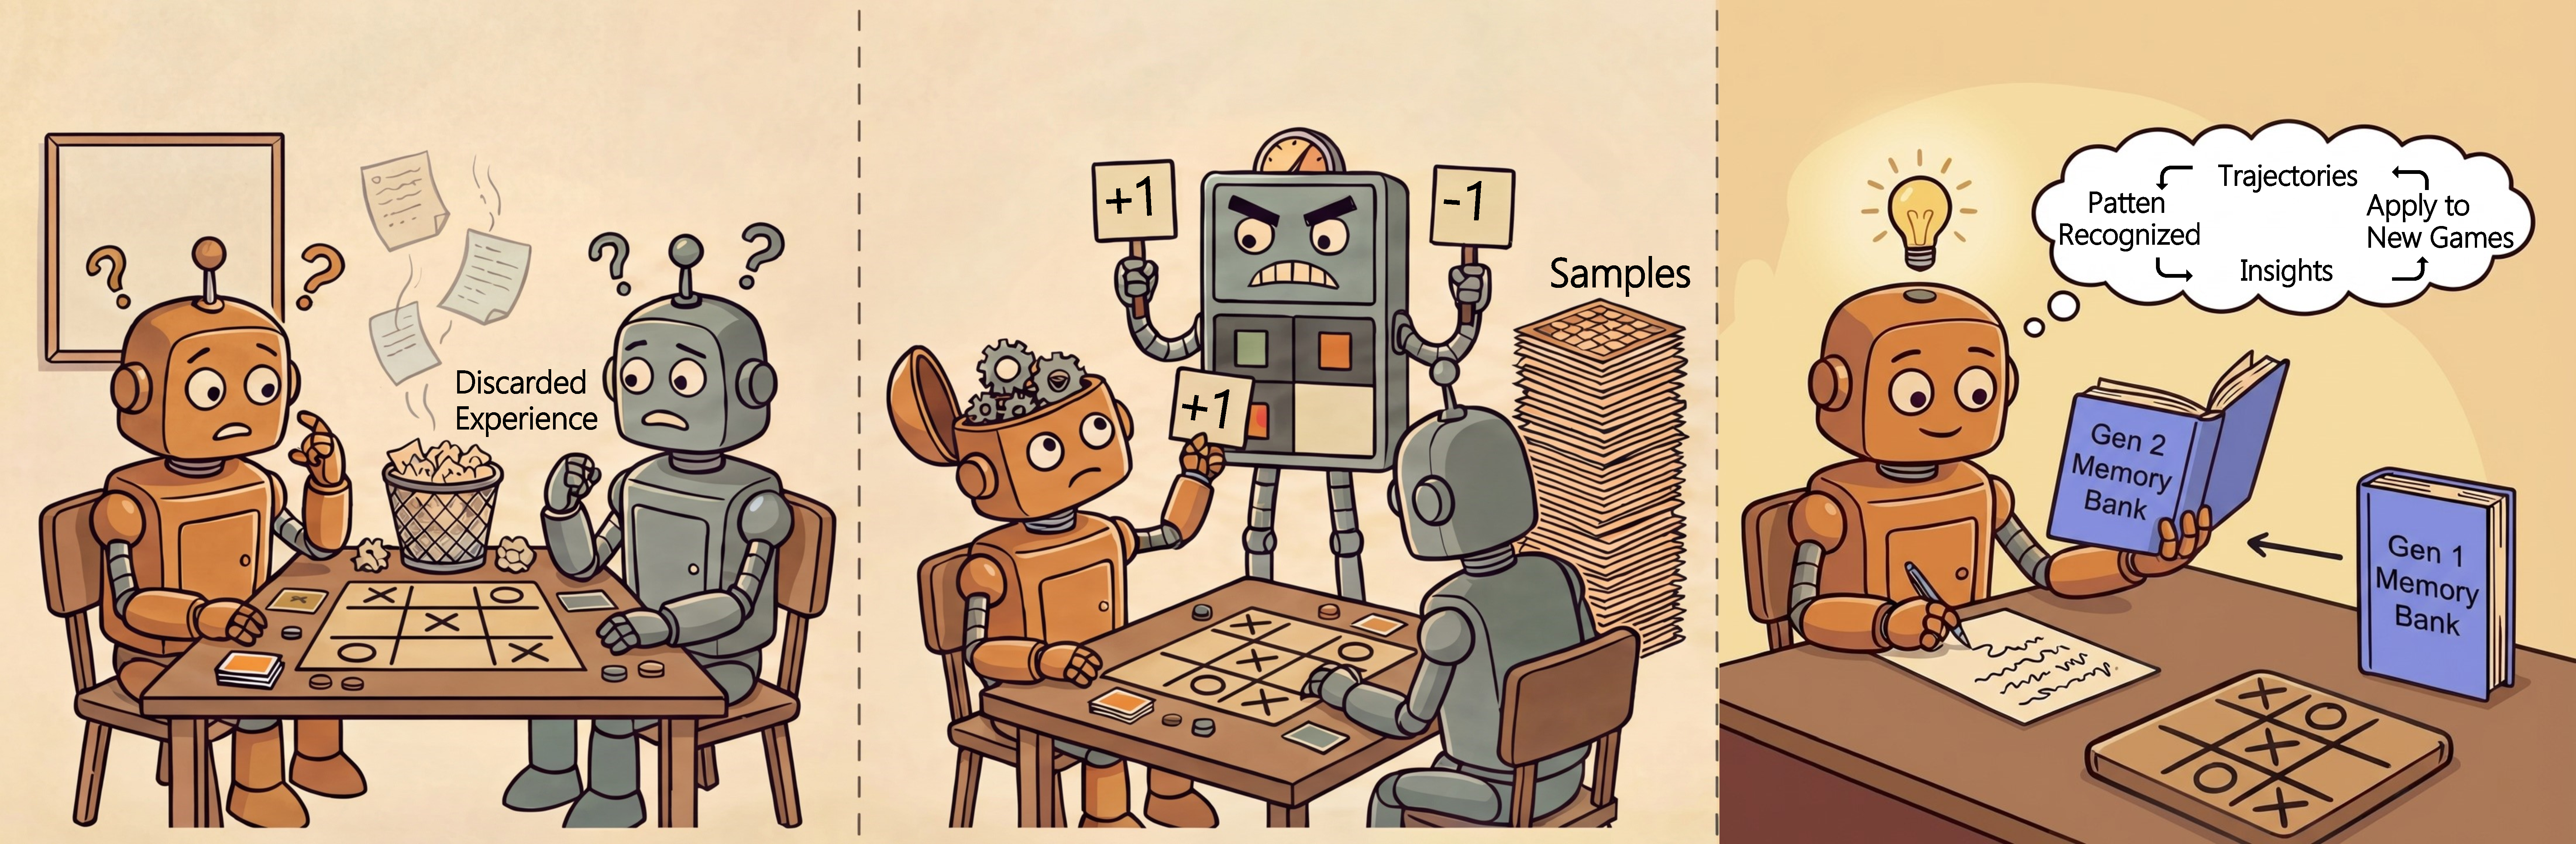
\includegraphics[width=\textwidth]{figures/comparison_visual.pdf}\\[2pt]
    \makebox[0.333\textwidth]{\small\textbf{(a) Self-Play Prompt Optimization}}%
    \makebox[0.333\textwidth]{\small\textbf{(b) Reinforcement Learning}}%
    \makebox[0.333\textwidth]{\small\textbf{(c) \NAME{} (Ours)}}
    \caption{\textbf{Three paradigms for learning in multi-agent LLM games.}
    \textbf{(a)}~Prompt optimization updates the system prompt each round
    through self-play, but game experience is not effectively retained across rounds,
    so strategic insights are lost across rounds.
    \textbf{(b)}~Reinforcement learning (RL) updates model weights through
    self-play but relies on outcome rewards, requiring large sample budgets.
    \textbf{(c)}~\NAME{} reflects on completed trajectories and accumulates
    reusable insights in a persistent memory bank across generations,
    enabling improvement without weight updates or external reward.}
    \label{fig:conceptual}
\end{figure*}
